\unchapter{Introduzione e Specifiche di Progetto}

%--------------------------------------------------------------------------------------------

In questa tesi viene discussa la progettazione di un sintetizzatore musicale compatibile con
lo standard modulare più diffuso al giorno d'oggi, ovvero Eurorack \cite{eurorack}. Più
precisamente si vuole realizzare un generatore di segnali che offra la possibilità di essere
controllato in tensione (Voltage Controlled Oscillator, o VCO in breve). In questo modo,
applicando dei segnali variabili nel tempo in ingresso al modulo, si è in grado di variare
dinamicamente la frequenza dei segnali in uscita.

Il range scelto per tale variazione comprende la fascia di frequenze dello spettro audio,
quindi da poche decine di $Hz$ a circa $7kHz$. Si desidera inoltre, la possibilità di
convertire a piacere il funzionamento del modulo in oscillatore a bassa frequenza (Low Frequency
Oscillator, o LFO), spostando quindi il range di frequenze disponibili da frazioni di
$Hz$ a qualche decina di $Hz$.
\medskip

\begin{figure}[ht]
    \centering
    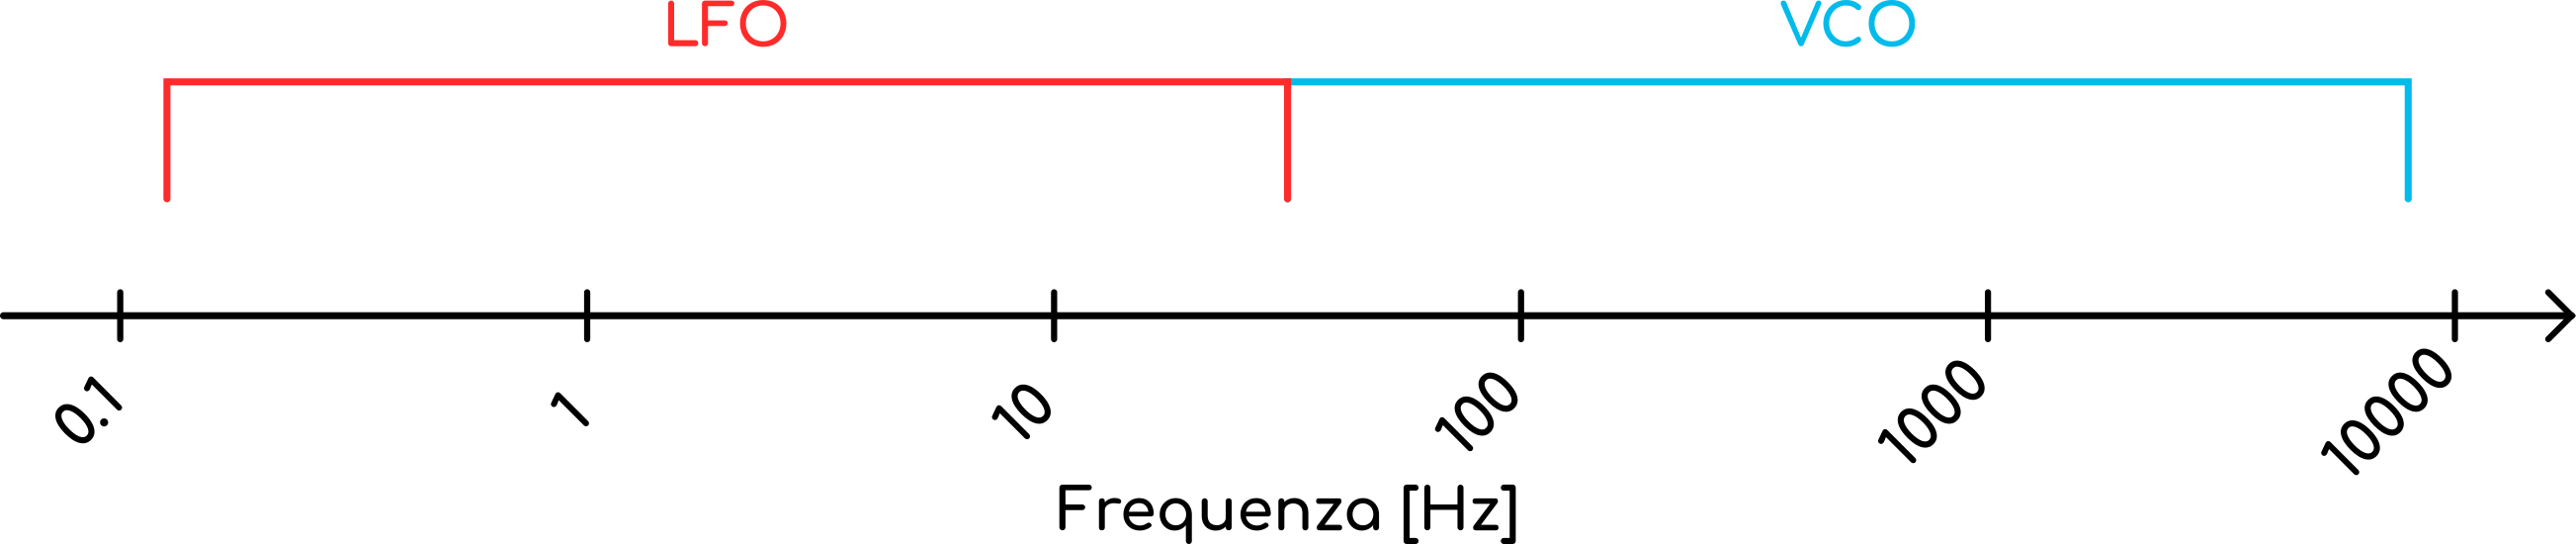
\includegraphics{graphs/functioning_range.png}
    \caption{Range di funzionamento approssimato, in scala logaritmica}
    \label{functioning_range}
\end{figure}

In modalità VCO quindi, il modulo produrrà dei segnali che attraverso un adeguato sistema
potranno essere ascoltati, mentre in modalità LFO il circuito produrrà dei segnali lentamente
variabili nel tempo, utili per la modulazione e il controllo di diversi parametri in altri
moduli eventualmente presenti nel sistema.

Le forme d'onda desiderate sono quelle base, ovvero:

\begin{itemize}
    \item Sinusoide;
    \item Onda Quadra;
    \item Triangolo;
    \item Rampa;
    \item Dente di sega (sebbene nel range VCO non risulti particolarmente differente dalla
          rampa in termini di suono, per quanto riguarda il funzionamento LFO la differenza
          è radicale, poichè il segnale viene solitamente utilizzato come modulante);
\end{itemize}

inoltre, come verrà illustrato più avanti, risulta piuttosto semplice anche estrarre un
segnale a impulso, anch'esso alla stessa frequenza di quelli già generati, per il controllo
di altri moduli o parametri.
\smallskip

Per quanto riguarda le specifiche sui livelli di tensione, si vogliono imporre i seguenti
intervalli di valori:

\begin{itemize}
    \item Segnali audio (i 5 elencati poco sopra): $\pm5V$;
    \item Segnali logici (impulso): $(0V,5V)$;
    \item Segnali di controllo (ingresso): $(0V,8V)$ in modalità $1V/Octave$, ovvero
          facendo in modo che ad un incremento di $1V$ corrisponda un raddoppio di frequenza,
          cioè un'ottava;
    \item Alimentazioni: $\pm12V$ e $+5V$;
\end{itemize}

Le specifiche sopra riportate sono prese dallo standard Eurorack.

Si desidera inoltre aggiungere delle manopole per il controllo del "volume" dei segnali
in ingresso e uscita, (ad eccezione dell'impulso) e delle manopole per il controllo
manuale della frequenza.

Mettendo assieme tutti questi dettagli possiamo abbozzare una interfaccia utente,
riportata in figura \ref{panel_explained}, in modo da rendere più chiaro al lettore il
prodotto finale.
\medskip

\begin{figure}[ht]
    \centering
    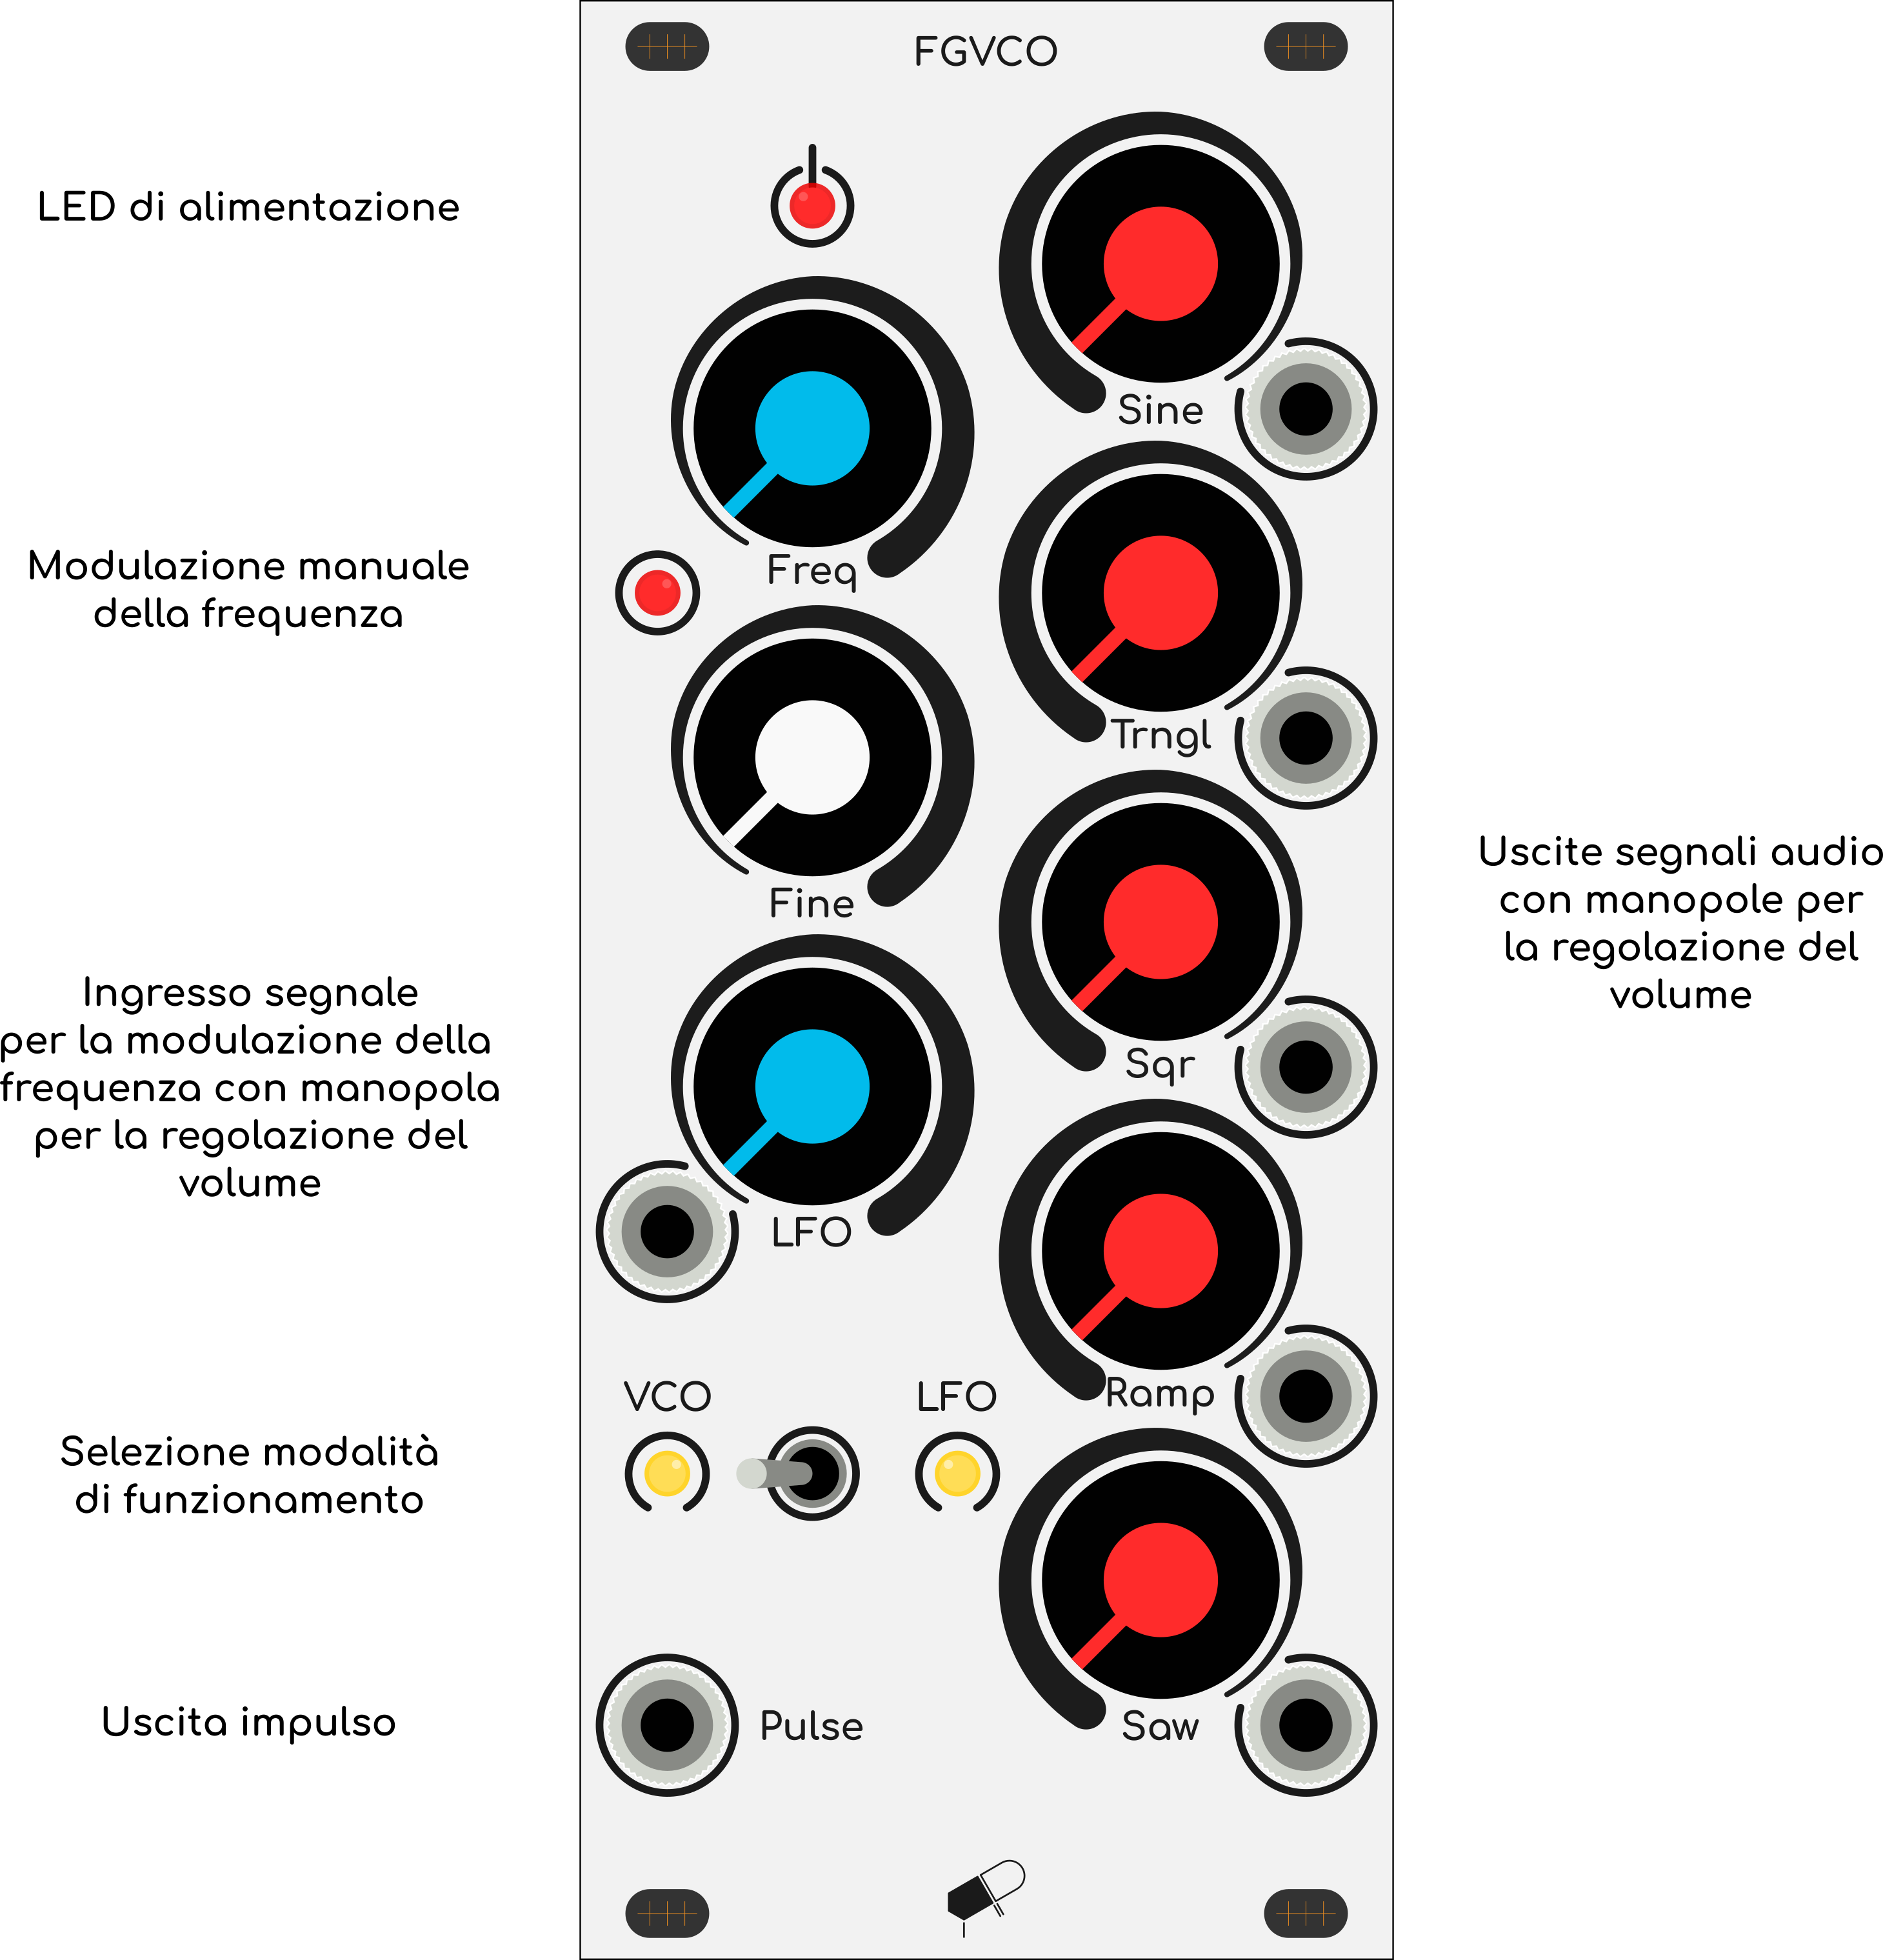
\includegraphics{misc/panel_explained.png}
    \caption{Pannello frontale del modulo}
    \label{panel_explained}
\end{figure}

Si decide di realizzare l'intero circuito senza l'utilizzo di microcontrollori o sistemi
programmabili. Tale scelta viene presa per mettere alla prova più competenze possibili tra
quelle acquisite durante gli anni di studio. Una soluzione possibile sarebbe infatti
impiegare un microcontrollore con dei campioni digitali molto fitti delle forme d'onda
desiderate.

%--------------------------------------------------------------------------------------------
